\chapter{Numerical Results}

In this section, we will show our pricing results for square root mean-reverting model and one heston one CEV model. We use Monte Carlo simulations as our benchmark as there's no existing pricing formulas for these two models.

\section{Volatility option prices under mean-reverting CEV model}

As mentioned in \ref{sec: 2.3}, we want to choose a nuisance parameter for our auxiliary model. In this case, our mis-pricing formula is given by

$$
\delta = \frac{1}{2} \sigma^{2} (V^{2\gamma} - V) \frac{\partial^{2} w}{\partial V^{2}} = \frac{1}{2} \sigma^{2} (V^{2\gamma-1} -1)V \frac{\partial^{2} w}{\partial V^{2}}
$$

We consider to choose $\hat{\sigma}$ such that

$$
\hat{\sigma}_{N}(x, t)=\arg \min _{\sigma}\left(w_{N}(x, t ; \sigma)-w_{0}(x, t ; \sigma)\right)^{2}
$$

\noindent Therefore, we let $\sigma = \sigma_{\text{CEV}}$

\noindent Res:


\begin{figure}[ht]
    \centering
    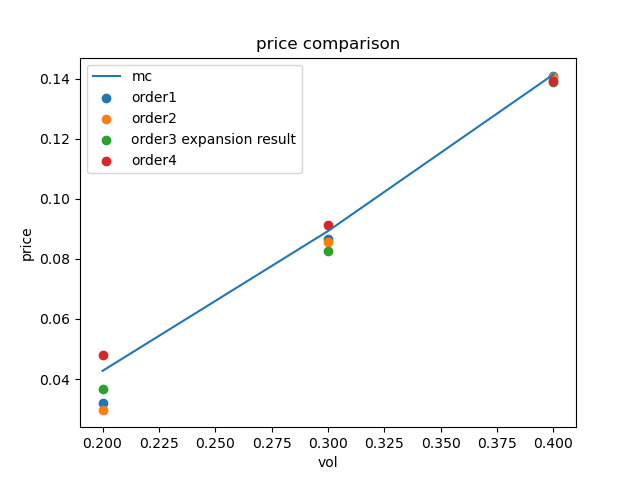
\includegraphics[width=10cm]{./figures/cev1.png}
    \caption{Call option price to volatility}\label{call2t}
\end{figure}